\chapter{Teoría de Sistemas Lineales}

\section{Matriz de transición de estados}
\subsection{Para LTI autónomo}
Sea un sistema LTI autónomo, es decir, sin entrada $u(t)$. Su solución $\tend{x}(t)$ se puede obtener utilizando transformación de Laplace:

\begin{align*}
    &\phantom{\Longrightarrow} \tend{\dot{x}}(t) =\tenq{A}\tend{x}(t)~/\mathcal{L}\{\cdot\}\\
    &\Longrightarrow s\tend{X}(s)-\tend{x_0} = \tenq{A}\tend{X}(s)\\
    &\Longrightarrow (s\tenq{I}-\tenq{A})\tend{X}(s) =\tend{x_0}\\
    &\Longrightarrow \tend{X}(s) = (s\tenq{I}-\tenq{A})^{-1}\tend{x_0}~/\mathcal{L}^{-1}\{\cdot\}\\
    &\Longrightarrow \tend{x}(t) = e^{\tenq{A}t}\tend{x_0}
\end{align*}

definiendo $\tenq{\phi}(t) = e^{\tenq{A}t}$ como la \emph{matriz de transición de estados}, la respuesta de los estados del sistema queda determinada por la siguiente expresión:

\begin{align*}
    \Longrightarrow \tend{x}(t) = \tenq{\phi}(t)\tend{x_0}
\end{align*}

Notar que $\tenq{\phi}(t)$ es una matriz que varía en función del tiempo.

\noindent \underline{Aparte}: Para entender qué significa $e^{\tenq{A}t}$ hay que recordar la Expansión de Taylor de una exponencial.\\

\noindent \underline{Definición}: Sea $f(t)$ una función suave y continua, su \emph{Expansión de Taylor} en torno a $t = \alpha$ es la siguiente:
\begin{align*}
    f(t) = f(\alpha)+\frac{\dot{f}(\alpha)}{1!}(t-\alpha)+\frac{\ddot{f}(\alpha)}{2!}(t-\alpha)^2+... = \sum_{n=0}^{\infty}{\frac{(t - \alpha)^n}{n!}\frac{d^n}{dt^n}f(t = \alpha)}   
\end{align*}
aplicando la expansión en una función exponencial en en torno a $\alpha = 0$:
\begin{align*}
    e^{at} = 1+at+\frac{1}{2!}a^2t^2+\frac{1}{3!}a^3t^3+... 
\end{align*}

La Expansión de Taylor de una exponencial también converge en torno a $\alpha = 0$ cuando se utiliza una matriz $\tenq{A}$ cuadrada. Por lo tanto, $\tenq{\phi}(t) = e^{\tenq{A}t}$ se puede calcular utilizando la siguiente serie:
\begin{align*}
    \tenq{\phi}(t) = e^{\tenq{A}t} = \tenq{I}+\tenq{A}t+\frac{1}{2!}\tenq{A}^2t^2+\frac{1}{3!}\tenq{A}^3t^3+...
\end{align*}

Notar que la expansión de Taylor de $\tenq{\phi}(t) = e^{\tenq{A}t}$ es una serie infinita. La serie finita se obtiene con el \emph{Teorema de Cayley-Hamilton} que se encuentra más adelante.

\underline{Nota}: $\tenq{\phi}(t)$ satisface la ecuación de estado:

\begin{align*}
    \Longrightarrow \tend{x}(t) &= \tenq{\phi}(t)\tend{x_0} = \left[\tenq{I}+\tenq{A}t+\frac{1}{2!}\tenq{A}^2t^2+...\right]\tend{x_0}\\
    \Longrightarrow \tend{\dot{x}}(t) &= \left[\tenq{A}+\frac{2}{2!}\tenq{A}^2t+...\right]\tend{x_0} =  \tenq{A}\left[\tenq{I}+\tenq{A}t+\frac{1}{2!}\tenq{A}^2t^2+...\right]\tend{x_0}\\
    \Longrightarrow \tend{\dot{x}}(t) &= \tenq{A}\tenq{\phi}(t)\tend{x_0}=\tenq{A}\tend{x}(t) \quad \text{(Ecuación de Estado)}
\end{align*}

\subsection{Para LTI no autónomo}
Si tenemos un sistema LTI no autónomo (es decir, con entrada u), la respuesta se encuentra de forma análoga:
\begin{align*}
    &\phantom{\Longrightarrow} \tend{\dot{x}}(t) = \tenq{A}\tend{x}(t)+\tenq{B}\tend{u}(t)\\
    &\Longrightarrow s\tend{X}-\tend{x_0} = \tenq{A}\tend{X}+\tenq{B}\tend{U}\\
    &\Longrightarrow (s\tenq{I}-\tenq{A})\tend{X} = \tend{x_0}+\tenq{B}\tend{U}\\
    &\Longrightarrow \tend{X}(s) = (s\tenq{I}-\tenq{A})^{-1} \tend{x_0}+(s\tenq{I}-\tenq{A})^{-1} \tenq{B}]tend{U}(s)\\
    &\Longrightarrow \tend{x}(t) = \tenq{\phi}(t)\tend{x_0}+\left[ \tenq{\phi}(t)\tenq{B} \right] \ast u(t)\\
    &\Longrightarrow \tend{x}(t) = \tenq{\phi}(t)\tend{x_0}+\int_0^t\tenq{\phi}(t-\tau)\tenq{B}\tend{U}(\tau)d\tau
\end{align*}

Notar que:
\begin{align*}
    \tenq{\phi}(t-\tau)&=e^{\tenq{A}(t-\tau)}\\
    &=e^{\tenq{A}t}\cdot e^{-\tenq{A}\tau}\\ 
    &=\tenq{\phi}(t)\tenq{\phi}(-\tau)
\end{align*} 

\noindent \underline{Aparte:} Sobre las propiedades de $\tenq{A}$, del problema de valores propios:
$$\tenq{A}\tend{v}=\lambda\tend{v}$$
donde $\tend{v}$ y $\lambda$ son el vector y valor propio asociado.
\begin{align*}
    \Longrightarrow \tenq{\phi}(t)\tend{v} &= \left[\tenq{I}+\tenq{A}t+\frac{1}{2!}\tenq{A}^2t^2+...\right]\tend{v}\\
    &= \tend{v}+\tenq{A}\tend{v}t+\frac{1}{2!}\tenq{A}^2\tend{v}t^2+... \\
    &= \tend{v}+\lambda\tend{v}t+\frac{1}{2!}\lambda^2\tend{v}t^2+... \\
    &= \left[ 1+\lambda t+\frac{\lambda^2}{2!}+\frac{\lambda^3}{3!}t^3 + ...\right]\tend{v}
\end{align*}
Si $\tend{x_0}=\tend{v}$, entonces $\tend{x}(t)=\tenq{\phi}(t)\tend{v}$\\

\noindent \underline{Aparte}: $\phi(t)$ una serie infinita ssi $\text{Re}(\lambda)<0$. Entonces el sistema LTI es estable.
\begin{align*}
    \lim_{t \to \infty} \phi(t)<\infty     
\end{align*}

\noindent \underline{Definición}: Una matriz $\tenq{A}$ se dice que es \textbf{Hurwitz} ssi los valores propios de $\tenq{A}$ tienen una parte real estrictamente negativa.


\section{Teorema de Cayley-Hamilton}
\underline{Teorema}: Sea una matriz $A\in\mathbb{R}^{n\times n}$, cuya ecuación característica $\Delta(\tenq{A}) = 0$ está dada por el siguiente polinomio de orden $n$:
\begin{align*}
    \Delta(\tenq{A})=\text{det}(s\tenq{I}-\tenq{A})=s^n+\alpha_{n-1}s^{n-1}+...+\alpha_1s+\alpha_0=0
\end{align*}
donde $\alpha_i\in\mathbb{R}$, $i\in [0,n-1]$, son los coeficientes del polinomio característico de $\tenq{A}$. Entonces, el teorema establece que la matriz $\tenq{A}$ también satisface la ecuación característica:
\begin{align*}
    \Delta (\tenq{A})=\tenq{A}^n+\alpha_{n-1}\tenq{A}^{n-1}+...+\alpha_1\tenq{A}+\alpha_0\tenq{I}=\tenq{0}
\end{align*}

Del teorema, podemos despejar $\tenq{A}^n$:
\begin{align*}
    \tenq{A}^n &= -\left[\alpha_{n-1}\tenq{A}^{n-1}+...+\alpha_1\tenq{A}+\alpha_0\tenq{I} \right]
\end{align*}

El poder de una matriz se escribe como una serie polinomial de orden igual al exponente del poder.\\

\par $\Longrightarrow$ Este resultado es útil para evaluar la matriz de transición $\phi(t)$
\begin{align*}
    \tenq{\phi(t)}=e^{\tenq{A}t}=\sum_{i=0}^\infty \beta_i(t)\tenq{A}^i \overset{\text{(C-H)}}{=} \sum_{i=0}^{n-1}\gamma_i(t)\tenq{A}^i
\end{align*}

\underline{Nota}: Este resultado es útil para evaluar $\phi(t)$ como una serie finita en términos de $A^i$.


\section{Equilibrio y Estabilidad}
\subsection{Plano de Fase}
El plano de Fase o diagrama de fase, es una representación gráfica de las trayectorias de un sistema dinámico en el tiempo, es decir, se puede observar como varían los estados en función del tiempo y entender mejor el comportamiento del sistema. También permite observar gráficamente la estabilidad. \\

Ejemplo: Considere el siguiente sistema dinámico LTI Autónomo de un grado de libertad.
\begin{figure}[H]
\centering
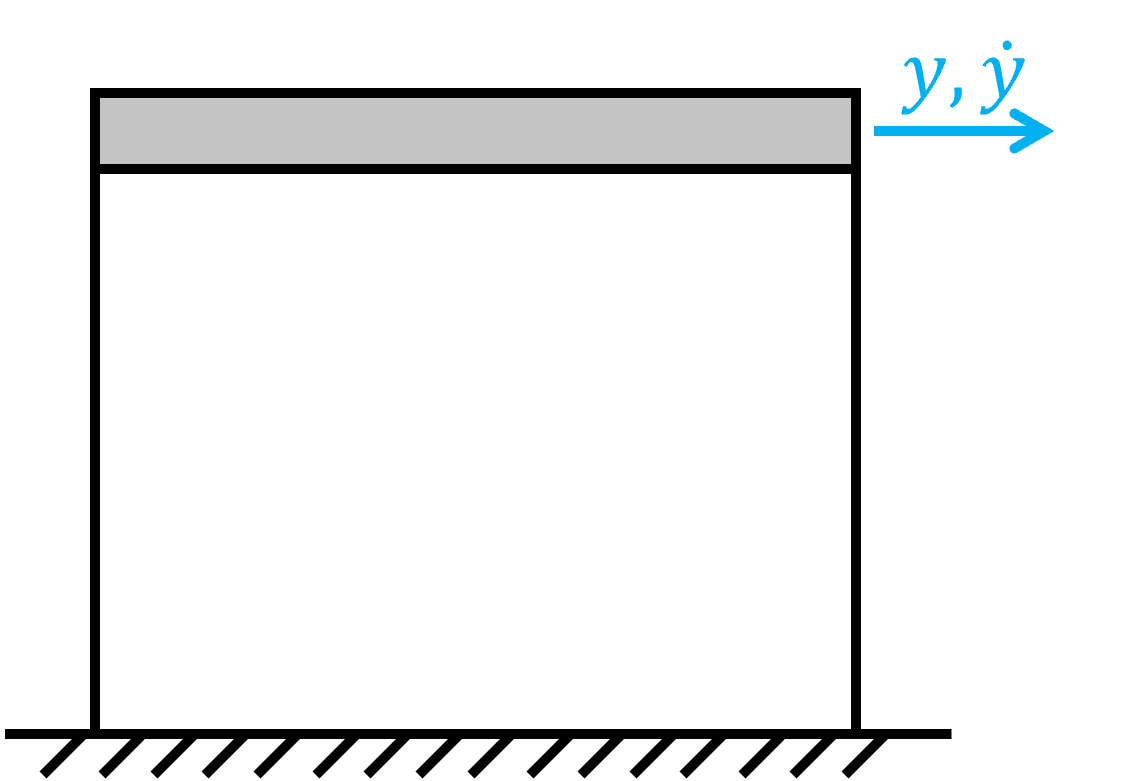
\includegraphics[scale=0.7]{Figuras/leccion11.png}
\end{figure}

\begin{align*}
    \Longrightarrow \tend{\dot{x}}(t) =\tenq{A}\tend{x}(t)
\end{align*}
donde $\tend{x}(t)=\begin{bmatrix} y(t)\\ \dot{y}(t) \end{bmatrix}$, con condiciones iniciales $y_0$, $\dot{y}_0$, se puede generar el siguiente diagrama de fase en el que se observa cómo varían los estados en el tiempo.
\begin{figure}[H]
\centering
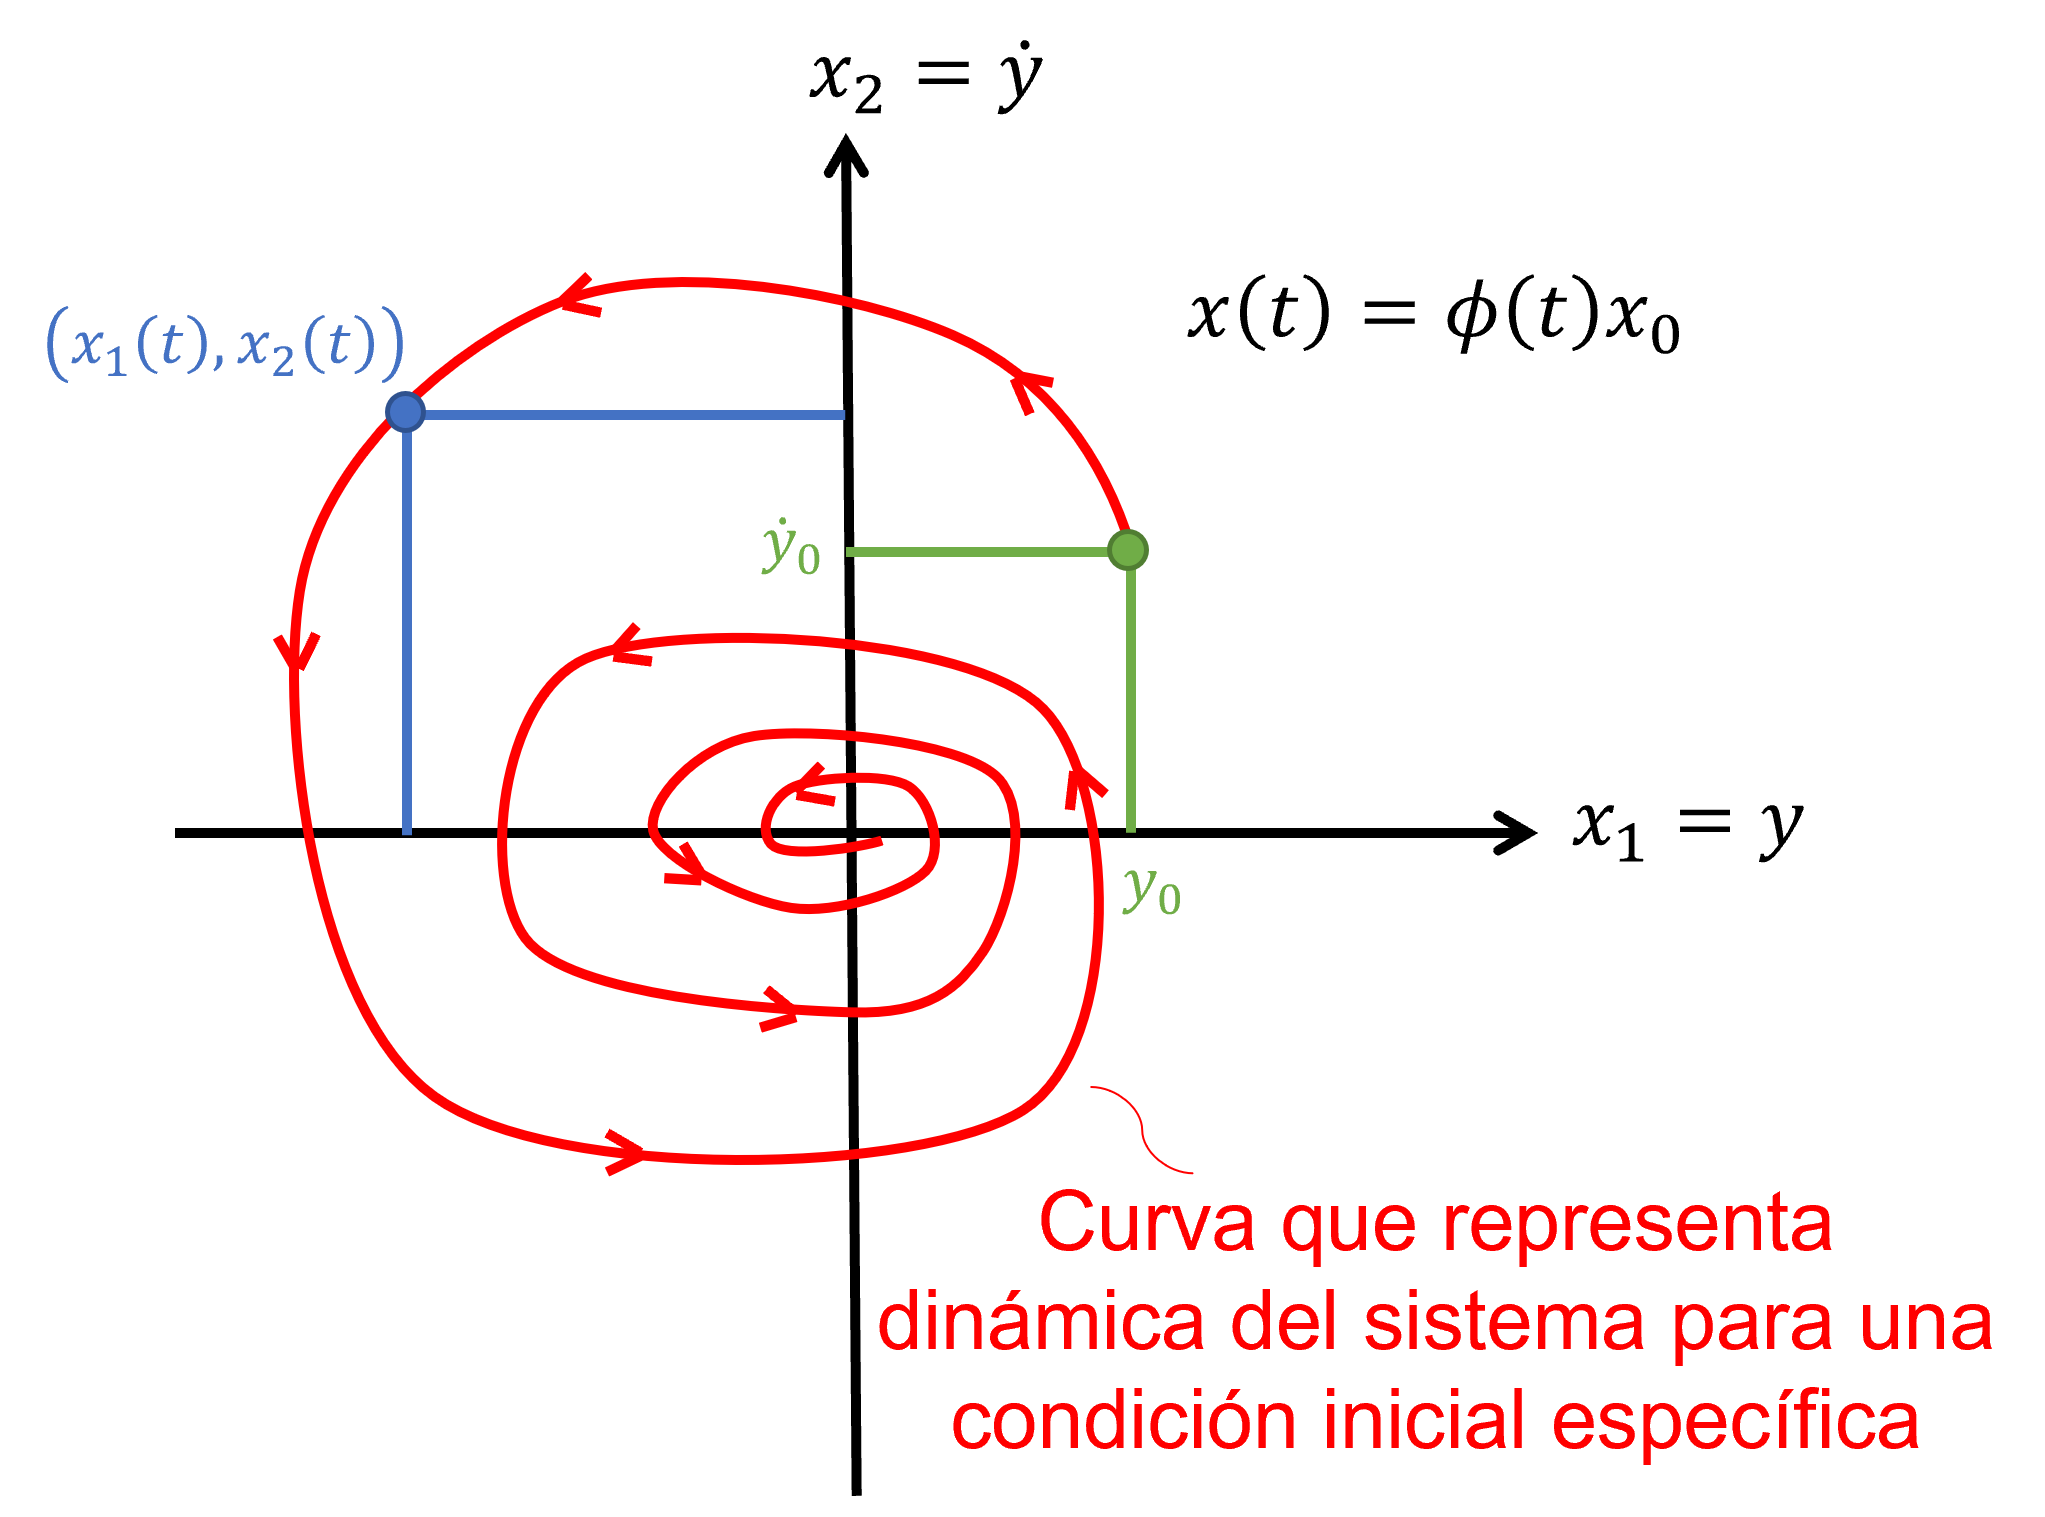
\includegraphics[scale=0.7]{Figuras/plano_de_fase.png}
\end{figure}
Notar que el diagrama de fase puede ser para cualquier vector de estados y no únicamente para dos estados como en este ejemplo.

\begin{figure}[H]
\centering
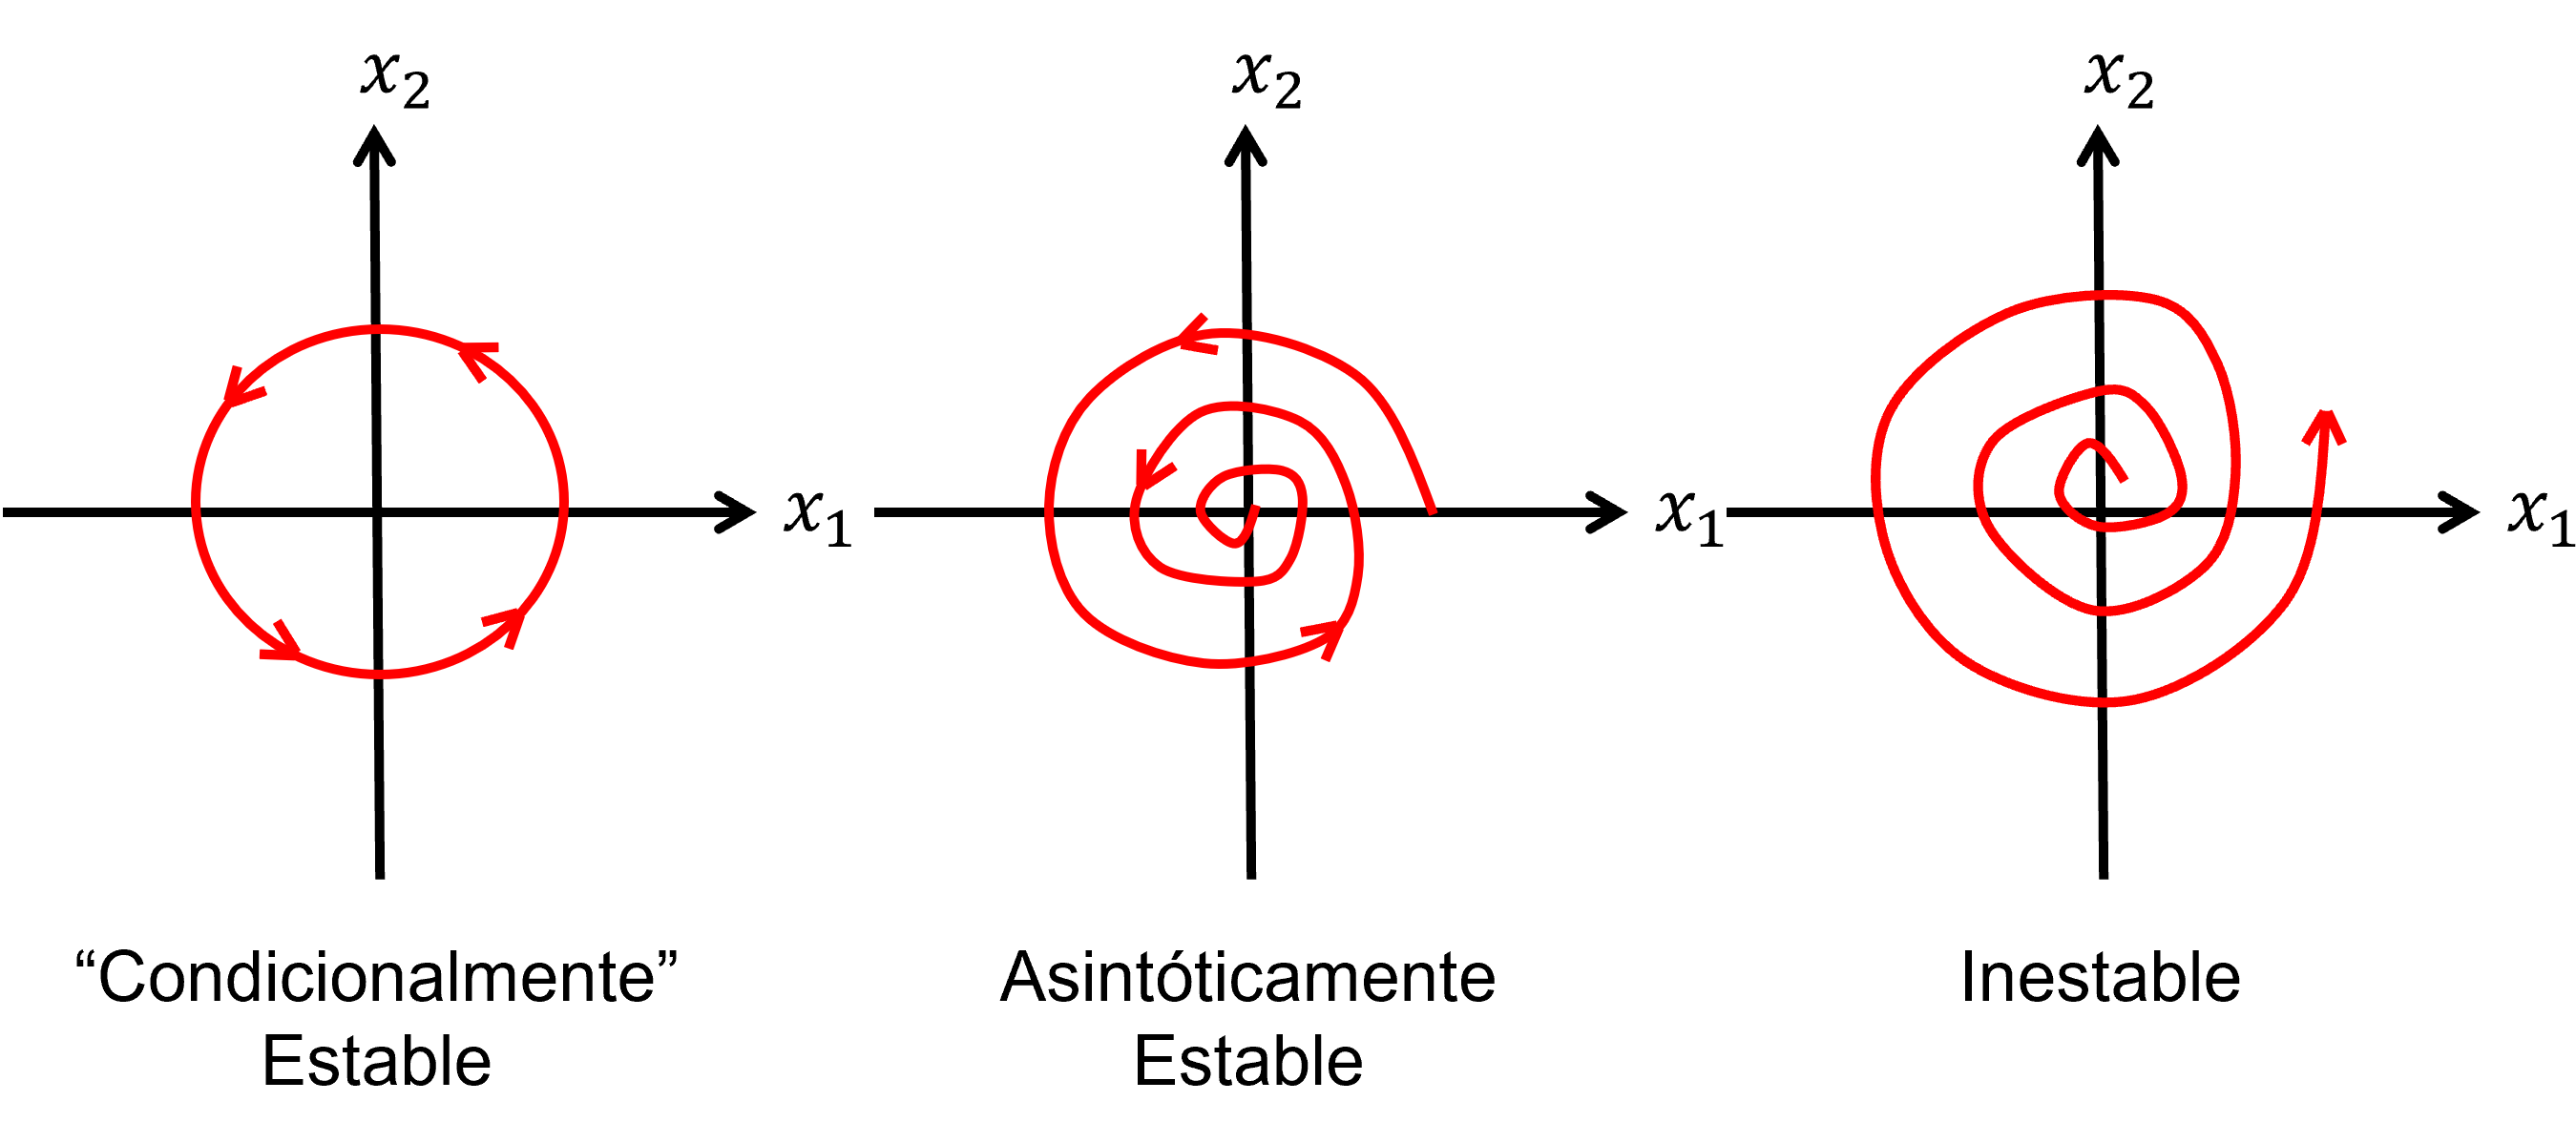
\includegraphics[scale=0.7]{Figuras/plano_de_fase.png_2.png}
\end{figure}

\subsection{Equilibrio}
Sea el sistema dinámico LTI en representación espacio-estado:
$$\tend{\dot{x}}=\tenq{A}\tend{x}+\tenq{B}\tend{u} $$

\noindent encontraremos una expresión para encontrar el estado en equilibrio $\tend{x_e}$. \\

\underline{Definición}: El equilibrio del sistema está dado por la condición de que $\tend{x}$ no cambia en el tiempo:
\begin{align*}
    \tend{\dot{x}} = \tend{0}
\end{align*}
Entonces, despejando el estado de equilibrio $\tend{x_e}$ desde el sistema LTI:
\begin{align*}
    &\Longrightarrow \tend{0}=\tenq{A}\tend{x_e}+\tenq{B}\tend{u_e} \\
    &\Longrightarrow \tend{x_e}=-\tenq{A}^{-1}\tenq{B}\tend{u_e} \Longrightarrow \text{ Estados de Equilibrio Estático}
\end{align*}

\noindent donde $\tend{x_e}$ es el vector de estado en equilibrio y $\tend{u_e}$ es el vector de entrada en el equilibrio, ambos constantes. \\

\underline{Notas}
\begin{itemize}
    \item Notar que si: $\tend{u_e}=\tend{0}\Longrightarrow\tend{x_e}=\tend{0}$.
    \item Los sistemas lineales presentan sólo un estado de equilibrio $\tend{x_e}$.
    \item No confundir: los estados de equilibrio $\tend{x_e}$ no son necesariamente \emph{estables}.
\end{itemize}

\subsection{Estabilidad de Lyapunov}
Sea un sistema dinámico LTI y autónomo: $\dot{x}=Ax$, $x(0) = x_0$ y $x_e$ un punto de equilibrio del sistema. Vamos a definir la estabilidad respecto a un punto de equilibrio.\\
\par \underline{Definición}: $x_e$ es estable en el sentido de Lyapunov si para cualquier $\varepsilon >0$ existe un $\delta >0$ tal que:
$$||x_0-x_e||<\delta\Longrightarrow ||x(t)-x_e||<\varepsilon, \quad \forall t>0$$
\begin{figure}[H]
\centering
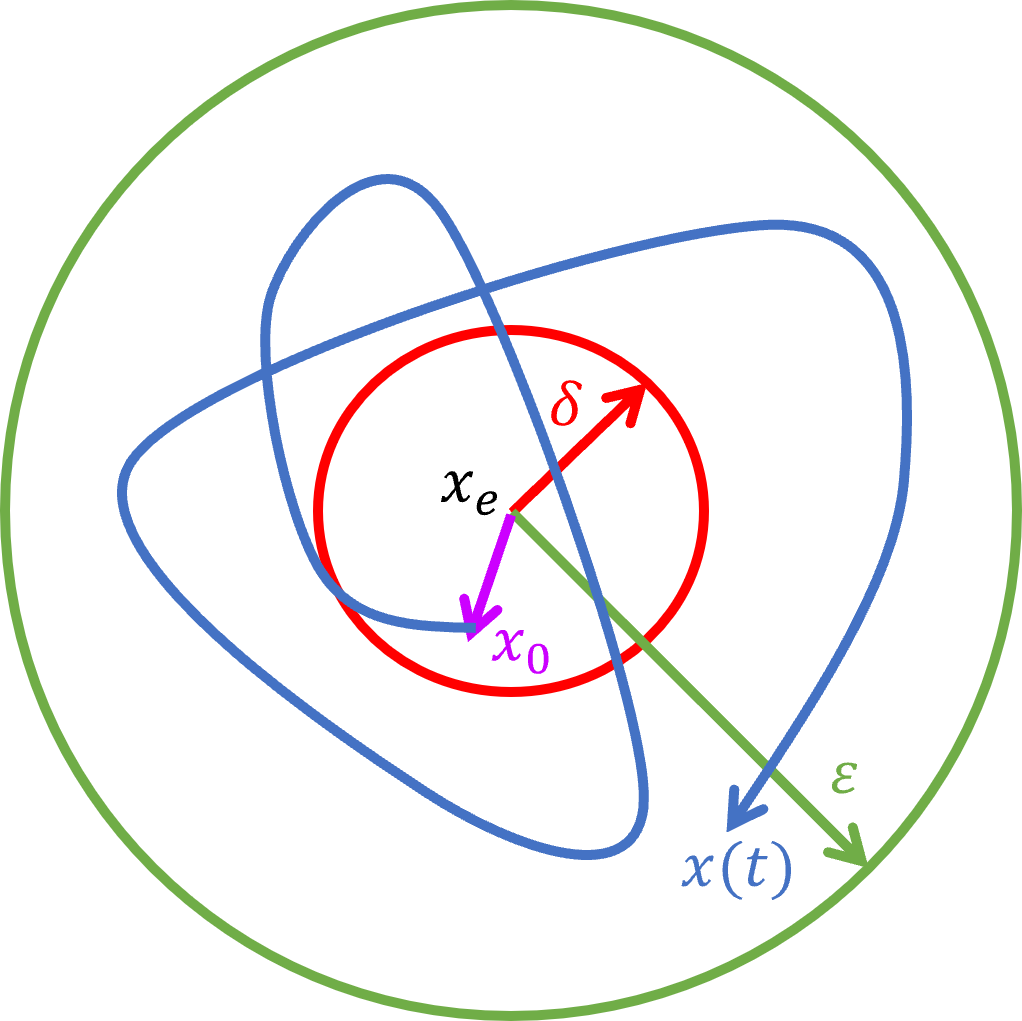
\includegraphics[scale=0.7]{Figuras/Lyapunov.png}
\end{figure}
* Mínima restricción que podemos imponer para satisfacer estabilidad.

\subsubsection{Definición Estabilidad Asintótica}
$x_e$ es asintóticamente estable si existe $\delta>0$ tal que:
\begin{itemize}
    \item $||x_0-x_e||<\delta$
    \item $x_e$ es estable en el sentido de Lyapunov
    \item $\lim_{t\to\infty}x(t)=x_e$
\end{itemize}
\begin{figure}[H]
\centering
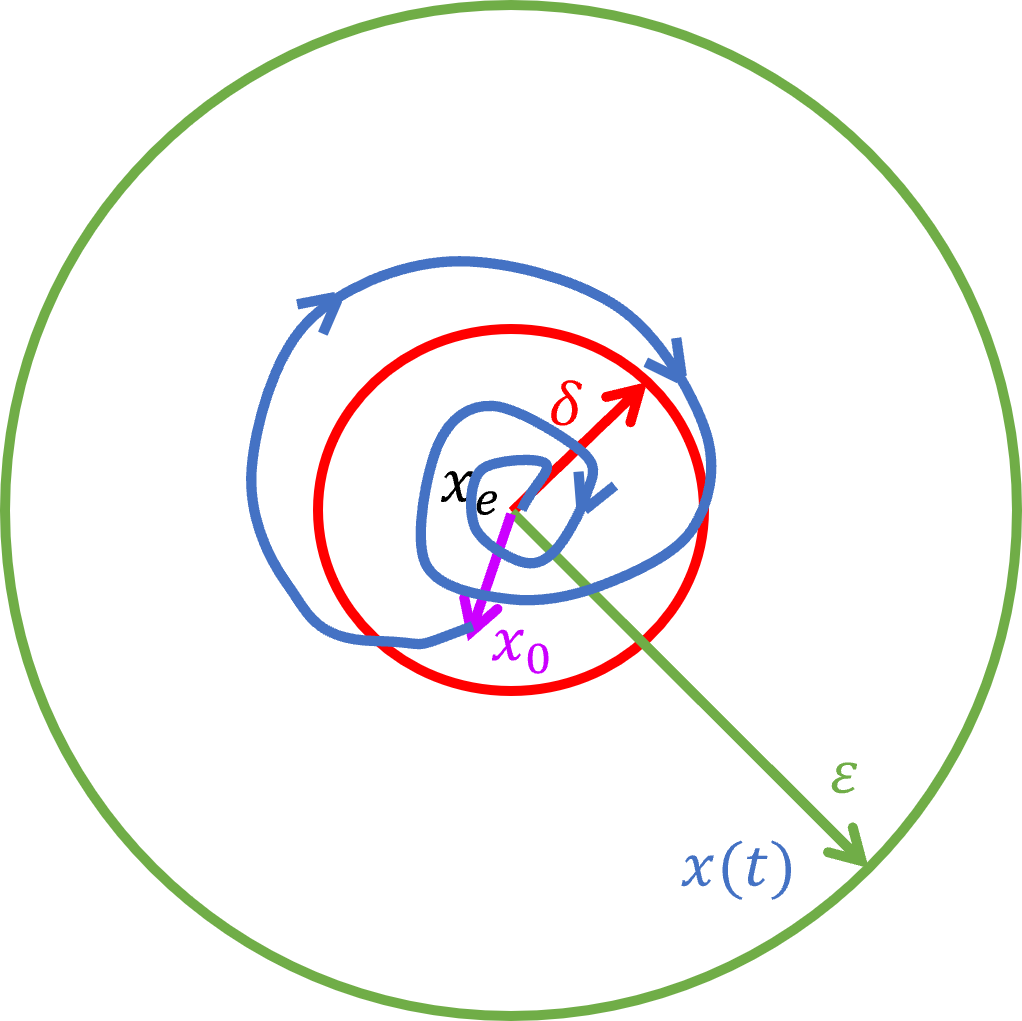
\includegraphics[scale=0.7]{Figuras/asintotica.png}
\end{figure}

\subsubsection{Definición Estabilidad Asintótica Global}
$x_e$ es estable asintótica global ssi es asintóticamente estable para $\delta \to \infty$.

\begin{table}[H]
    \centering
    \begin{tabular}{c|c|c|c|}
                & \raisebox{-\totalheight}{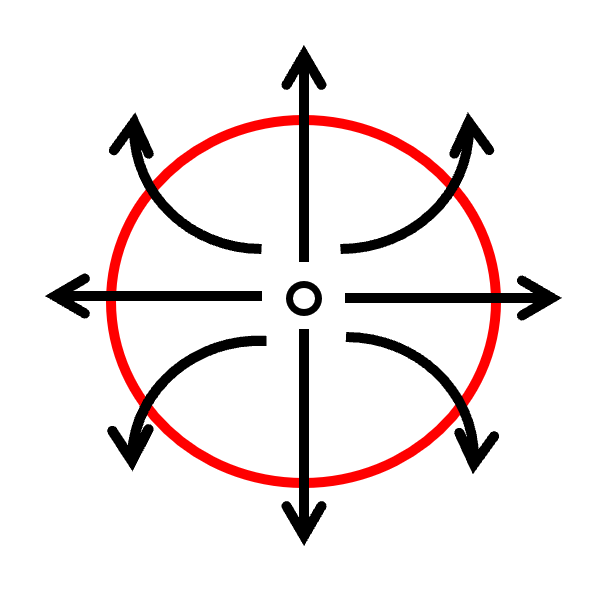
\includegraphics[scale=0.5]{Figuras/global1.png}} & \raisebox{-\totalheight}{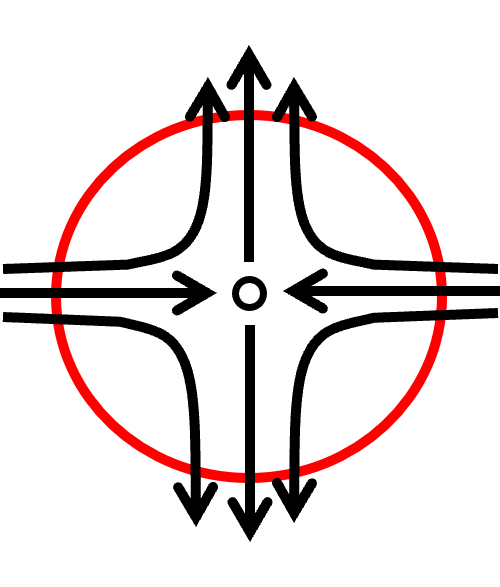
\includegraphics[scale=0.5]{Figuras/global2.png}} & \raisebox{-\totalheight}{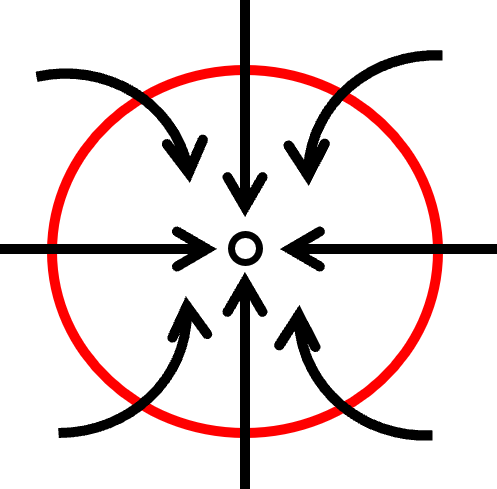
\includegraphics[scale=0.5]{Figuras/global3.png}}\\ \hline
         Estable & \xmark & \xmark & \cmark\\
         Asint. Est. & \xmark & \xmark &\cmark \\
         Goblal Asint. Est. & \xmark & \xmark & \textbf{???}
    \end{tabular}
\end{table}


\subsubsection{Límites de Estabilidad para sistemas LTI}
Sea el sistema LTI autónomo $\dot{x}(t)=Ax(t)$, cuya solución es $x(t)=\phi(t)x_0$ y $x_e$ un estado de equilibrio. Se requiere analizar la estabilidad en el sentido de Lyapunov. Por lo cual hay que analizar las normas $||x(t) - x_e||$ y $||x_0 - x_e||$ \\

\par Suponiendo que $\phi(t)$ es finita, es decir, $||\phi(t)||=||e^{At}||\leq\beta<\infty$. Se tiene que la siguiente diferencia de vectores de estados:
\begin{align*}
    x(t)-x_e &= \phi(t)x_0-x_e\\
    &= \phi(t)x_0-\phi(t)x_e\\
    &= \phi(t)[x_0-x_e]
\end{align*}

Para este sistema, notar que si $x_0 = x_e$, entonces $x(t)=x_e$, es decir, si el estado inicial es un estado de equilibrio (por ejemplo, el reposo) y si no existen exitaciones, entonces los estado $x(t)$  se mantendrán constantes e igual a al estado de equilibrio $x_e$, para $\phi(t)x_e=x_e$.\\

Entonces, extrayendo la norma de la expresión anterior:
\begin{align*}
    ||x(t)-x_e||=||\phi(t)[x_0-x_e]||\leq||\phi(t)||\cdot||x_0-x_e||
\end{align*}
Luego, si $||x_0 - x_e||<\delta$
\begin{align*}
    &\Longrightarrow ||x(t)-x_e||\leq ||\phi(t)|| \delta
\end{align*}
Si definimos $||\phi(t)||\delta = \varepsilon$:
\begin{align*}
    &\Longrightarrow ||x(t) - x_e|| \leq \varepsilon
\end{align*}

Por lo tanto, si $\phi(t)$ es finito, implica que $x_e$ es estable en el sentido de Lyapunov. 
$\phi(t)$ es finito si y solo si $A$ es Hurwitz:
\begin{align*}
    \text{Re}\left(\text{eig}(A)\right)<0\Longrightarrow \text{Estabilidad}
\end{align*}

\subsubsection{Función Candidata de Lyapunov}
\underline{Definición}: Sea una función $V(x)$, $\mathbb{R}^n\to \mathbb{R}$, tal que: 
\begin{itemize}
    \item $V(x_e)=0$
    \item $V(x)>0$, $\forall x\neq x_e$ ($V$ es una función definida positiva)
    \item $V$ y su primera derivada son finitas
\end{itemize}

Entonces, $V(x)$ es una función candidata de Lyapunov.\\
\par \underline{Teorema}: Si $V(x)$ s una función candidata de Lyapunov para $x_e$ en una región $\Omega$ vecina a $x_e$:
\begin{itemize}
    \item[a)] $x_e$ es estable en el sentido de Lyapunov si:
    $$\frac{dV(x)}{dt}\leq 0, ~\forall x\in \Omega $$
    \item[b)] $x_e$ es asintóticamente estable si:
    $$\frac{dV(x)}{dt}< 0, ~\forall x\in \Omega$$
    \item[c)] $x_e$ es global asintóticamente estable si:
    $$\frac{dV(x)}{dt}< 0, ~\forall x\in \Omega$$
    donde $\Omega \in \mathbb{R}^n$ y $V(x)$ no tiene límite radial.
\end{itemize}

\underline{Ilustración}: Sean $x=\begin{bmatrix}x_1\\ x_2\end{bmatrix}$, $x\in \mathbb{R}^2$, $x_e=0$ y $V(x)=x^\top x$ una función candidata de Lyapunov.

\begin{figure}[H]
\centering
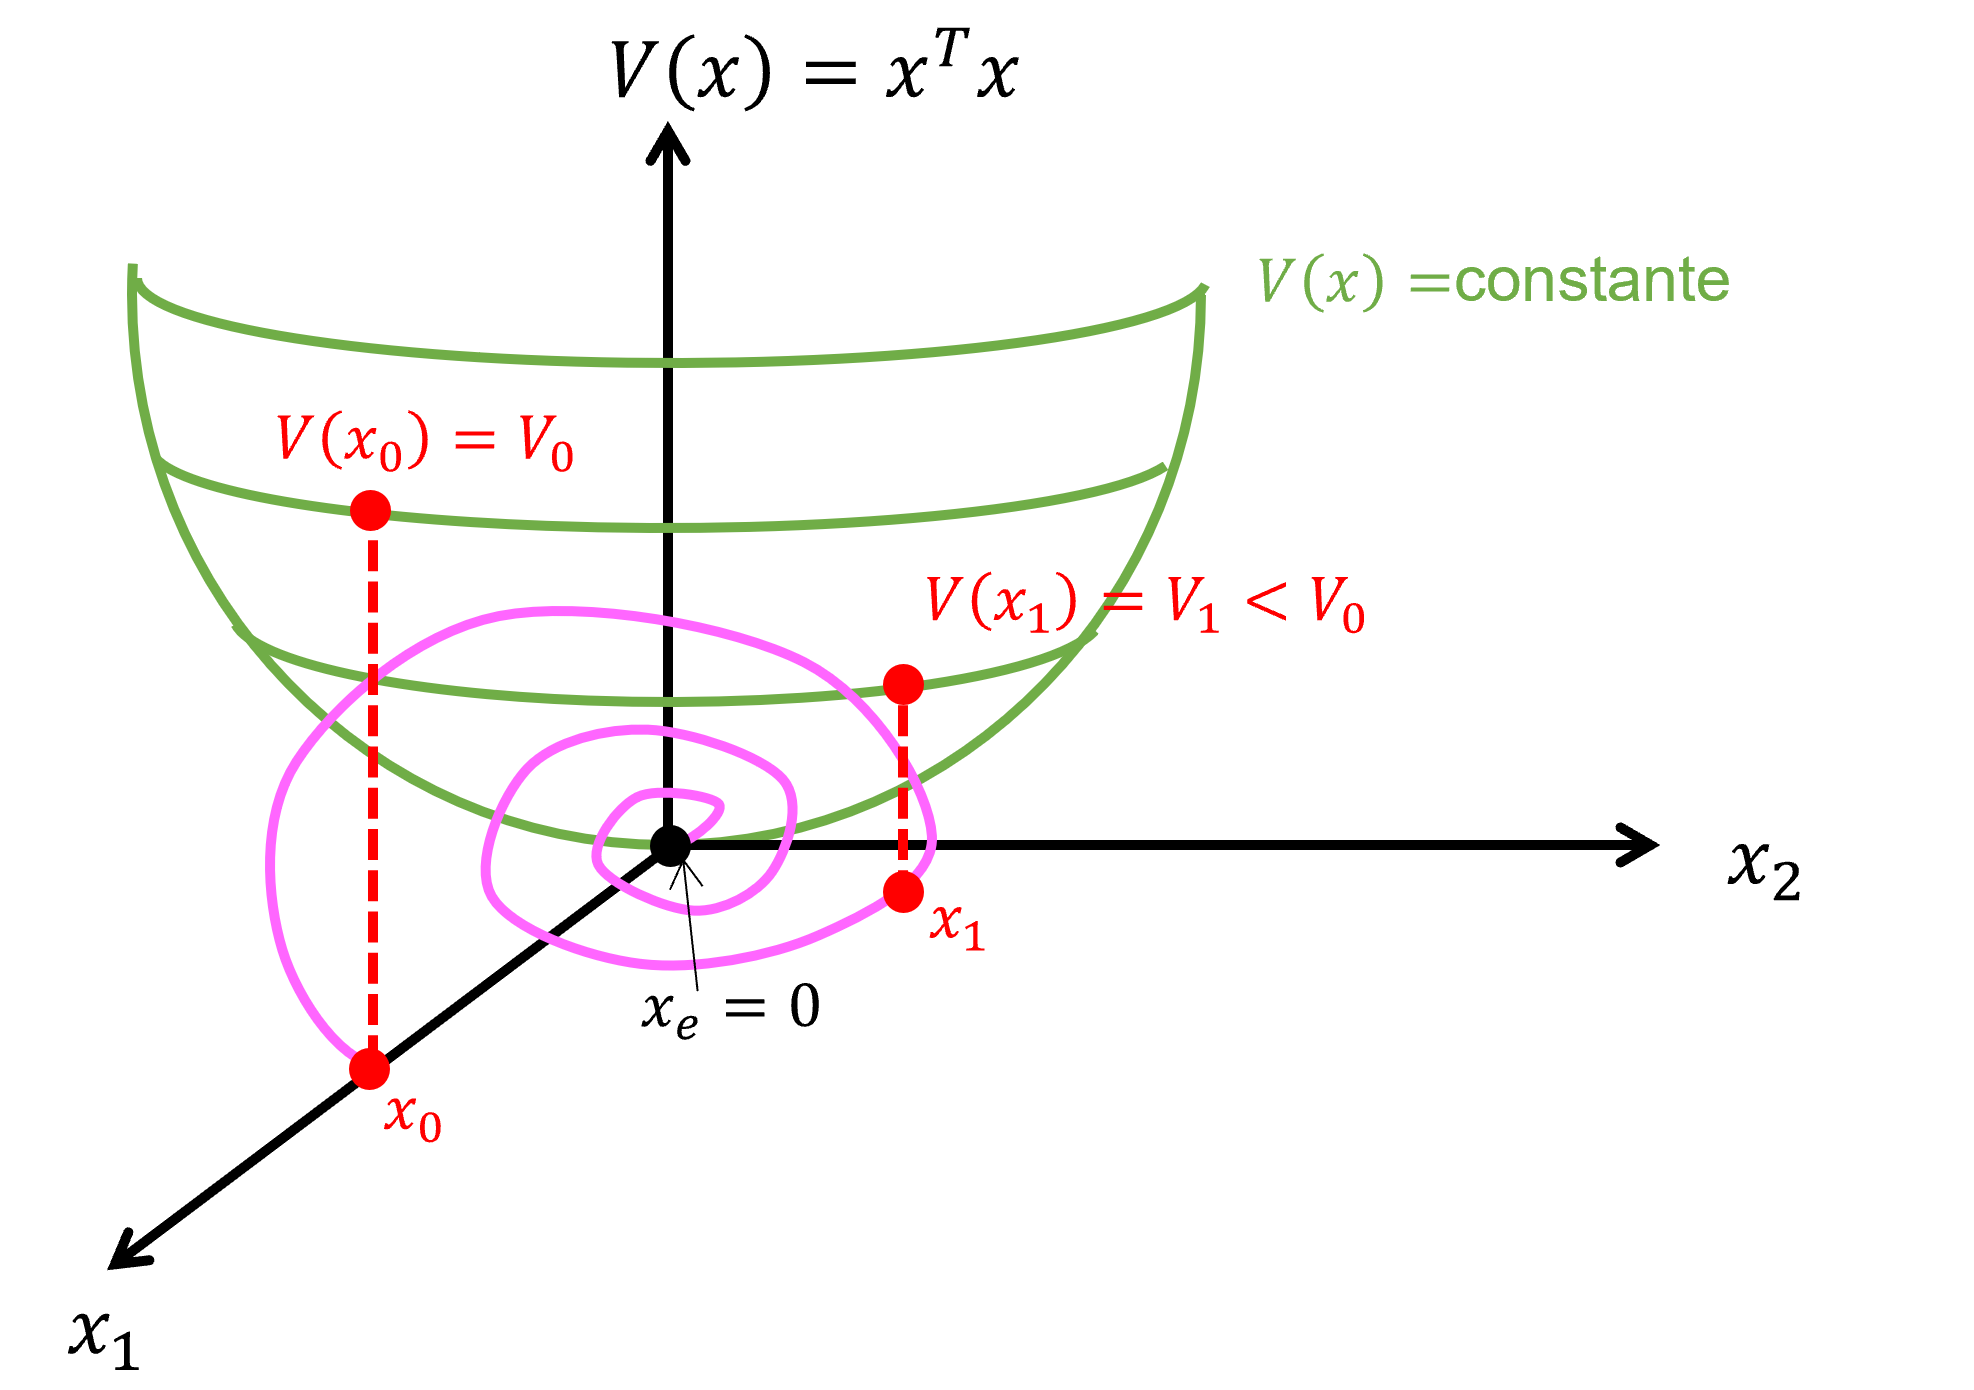
\includegraphics[scale=0.7]{Figuras/ilu_lyapunov.png}
\end{figure}

Notar que:
\begin{align*}
    \frac{dV(x)}{dt} < 0   
\end{align*}

Ocupando $V=V(x(t))$. Entonces:
\begin{align*}
    \frac{dV}{dt} &= \frac{\partial V}{\partial x}\cdot \frac{\partial x}{\partial t}  \quad \text{Regla de la cadena}\\
    &= \sum_{i=1}^n \frac{\partial V}{\partial x_i}\cdot\frac{\partial x_i}{\partial t}\\
    &= \begin{bmatrix}\frac{\partial V}{\partial x_1} &...& \frac{\partial V}{\partial x_n}\end{bmatrix}\begin{bmatrix}\dot{x}_1\\ \vdots \\ \dot{x}_n\end{bmatrix}\\
    &= \nabla V\cdot \dot{x}
\end{align*}

\begin{align*}
    \frac{dV}{dt}=\nabla V\cdot \dot{x}<0, ~\forall t
\end{align*}

Dibujemos una línea de contorno de $V(x)$: \\
\begin{figure}[H]
\centering
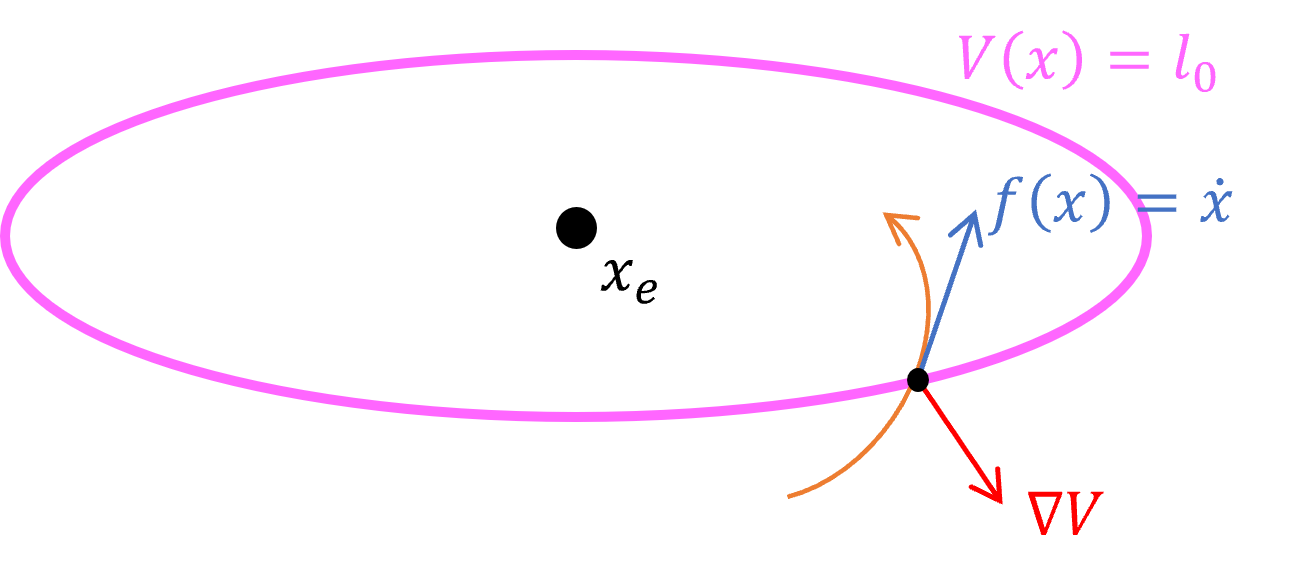
\includegraphics[scale=0.7]{Figuras/ilu_lyapunov2.png}
\end{figure}

\begin{align*}
    \nabla V\cdot f(x)<0 \Longrightarrow \text{Entonces el sistema se acerca a } x_e   
\end{align*}

$\Longrightarrow x_e$ es un punto de atracción o \emph{sumidero}.\\

\par Para el sistema LTI autónomo $\dot{x}=Ax$, y sea $V(x)=x^\top Px$, donde $P$ es una matriz definida positiva y simétrica.
$$\frac{dV}{dt}=\nabla V\cdot \dot{x}<0 $$ 

para un sistema asintóticamente estable.\\
\begin{align*}
    \nabla V=\frac{\partial}{\partial \tend{x}} (\tend{x}^\top \tenq{P}\tend{x}) = 2\tenq{P}\tend{x} \quad \text{Por demostrar}
\end{align*}

Entonces:
\begin{align*}
    \frac{dV}{dt} &= (2Px)^\top (Ax)= (2x^\top P^\top)(Ax)\\
    &= (x^\top P^\top)(Ax)+x^\top P^\top Ax\\
    &= (Px)^\top(Ax)+x^\top PAx\\
    &= (Ax)^\top(Px)+x^\top PAx\\
    &= x^\top A^\top Px+x^\top PAx\\
    &= x^\top (A^\top P+PA)x<0
\end{align*}

Por lo tanto, $A^\top P+PA \prec 0$ debe ser una matriz definida negativa para que el sistema sea asintóticamente estable.\\
\par Sea $Q$ una matriz definida positiva y simétrica, tal que:
\begin{align*}
    &\phantom{\Longrightarrow} A^\top P+PA = -Q\\
    &\Longrightarrow A^\top P+PA+Q = \emptyset \quad \text{Ecuación de Lyapunov}
\end{align*}

\underline{Teorema}: Dados $Q \succ 0$ y simétrico, existe un $P\succ 0$ simétrico que satisface:
$$A^\top P+PA+Q=\emptyset $$

entonces, $\dot{x}=Ax$ es asintóticamente estable.

\section{Controlabilidad}
% La controlabilidad es una propiedad de cualquier sistema dinámico.\\

Sea un sistema LTI: $\dot{x}=Ax+Bu$, $x\in \mathbb{R}^n$, $u\in\mathbb{R}^p$. Buscamos $u(t)$ tal que los estados vayan de $x(t)$ a cero en un tiempo finito $t_1$. \\
Recordar que la solución de un sistema LTI no autónomo es:
\begin{align*}
    x(t)=\phi(t)x_0+\int_0^t \phi(t-\tau)Bu(\tau)d\tau    
\end{align*}
Luego, si $x(t_1) = 0$
\begin{align*}
    0=\phi(t_1)x_0+\int_0^{t_1} \phi(t_1-\tau)Bu(\tau)d\tau
\end{align*}

Considerando la propiedad: $\phi(t_1-\tau)=e^{A(t_1-\tau)}=e^{At_1}\cdot e^{-A\tau}=\phi(t_1)\phi(-\tau)$. Entonces:

\begin{align*}
    0 &=\phi(t_1)\left[x_0+\int_0^{t_1}\phi(-\tau)Bu(\tau)d\tau\right] \\
    \Longrightarrow -x_0 &= \int_0^{t_1}\phi(-\tau)Bu(\tau)d\tau
\end{align*}

Por el teorema de Cayley-Hamilton:
\begin{align*}
    \phi(-\tau)=m_0(\tau)I+m_1(\tau)A+m_2(\tau)A^2+...+m_{n-1}(\tau)A^{n-1}
\end{align*}

Entonces:
\begin{align*}
    -x_0 &= \int_0^{t_1}\left[m_0(\tau)B+m_1(\tau)AB+m_2(\tau)A^2B+...+m_{n-1}(\tau)A^{n-1}B \right]u(\tau)d\tau\\
    \Longrightarrow -x_0 &= \int_0^{t_1} \sum_{j=0}^{n-1}A^jBm_j(\tau)u(\tau)d(\tau)\\
    \Longrightarrow -x_0 &= \sum_{j=0}^{n-1}A^jB \int_0^{t_1} m_j(\tau)u(\tau)d\tau
\end{align*}

Cada término de la integral es un vector constante de dimensión $p\times 1$
\begin{align*}
    \Longrightarrow v_j := \int_0^{t_1}m_j(\tau)u(\tau)d\tau
\end{align*}

\begin{align*}
    \Longrightarrow -x_0 &= \sum_{j=0}^{n-1}A^jBv_j =Bv_0+ABv_1+...+A^{n-1}Bv_{n-1}\\
     \Longrightarrow -x_0 &= \left[
    \begin{array}{c|c|c|c|c}
     B & AB & A^2B & ... & A^{n-1}B
    \end{array}\right] \left[
    \begin{array}{c}
     v_0\\ \hline v_1 \\ \hline v_2 \\ \hline \vdots \\ \hline v_{n-1} 
    \end{array}\right]
\end{align*}

Por lo tanto, se define la \emph{Matriz de Controlabilidad} $\mathcal{C}$:
\begin{align*}
    \mathcal{C}=\left[
    \begin{array}{c|c|c|c|c}
     B & AB & A^2B & ... & A^{n-1}B
    \end{array}\right]
\end{align*}

Este resultado indica que cualquier vector $-x_0$ puede ser expresado como una combinación lineal de las columnas de la matriz $\mathcal{C}$. Esta matriz $\mathcal{C}$ debe tener rango igual a $n$ para escribir $-x_0 \in \mathbb{R}^n$.\\

\underline{Por lo tanto, un sistema LTI es controlable ssi $\text{rank}(\mathcal{C})=n$}. \\

\underline{Nota}: Si $\text{rank}(\mathcal{C})= n_e < n$, entonces el sistema tiene no más de $n_e$ estados controlables.\\
\par \underline{Definición}: Si el sistema tiene estados inestables, pero controlables, entonces se dice que estos estados son \textbf{estabilizables}. Por lo tanto, puede diseñar $u(t)$ tal que el sistema cerrado tenga todos sus estados estables.\\

\underline{Nota}: Sea el sistema LTI, $\dot{x}=Ax+Bu$, y sea $T$ una matriz de transformación tal que $x=Tz$, donde $\dot{z}=A_cz+B_cu$, es una realización CCF. Entonces, el sistema es controlable ssi $T$ existe.

\section{Observabilidad}
Asuma el sistema LTI autónomo:
\begin{align*}
    \dot{x} &= Ax, \quad x\in\mathbb{R}^n\\
    y &= Cx, \quad y\in\mathbb{R}^r
\end{align*}

\begin{align*}
    \begin{array} {|c|}
  \hline \text{Caja}\\ 
  \text{Negra} \\
  \hline 
\end{array} \longrightarrow y\in\mathbb{R}^r
\end{align*}

Sabemos que la solución $x(t)$: 

\begin{align*}
    x(t) = \phi (t) x_0 \Longrightarrow y(t) = C x(t) = C \phi (t) x_0    
\end{align*}

Además, utilizando el Teorema de Cayley-Hamilton:
\begin{align*}
    y(t) &= Ce^{At}x_0\\
    y(t) &= C\left[l_0(t)I+l_1(t)A+l_2(t)A^2+...+l_{n-1}(t)A^{n-1} \right]x_0\\
    y(t) &= \left[
    \begin{array}{c|c|c|c|c}
     l_0(t) & l_1(t) & l_2(t) & ... & l_{n-1}(t)
    \end{array}\right] \left[
    \begin{array}{c}
     C\\ \hline CA \\ \hline CA^2 \\ \hline \vdots \\ \hline CA^{n-1} 
    \end{array}\right] x_0
\end{align*}

Se define:
\begin{align*}
    \mathcal{O}=\left[
    \begin{array}{c}
     C\\ \hline CA \\ \hline CA^2 \\ \hline \vdots \\ \hline CA^{n-1} 
    \end{array}\right] \quad \text{Matriz de observabilidad}
\end{align*}

Si $\mathcal{O}$ no es de rango completo, entonces podemos elegir $x_0\neq 0$ tal que $y(0)=0$, porque $t_0$ puede producir el mismo resultado. \\
\par \underline{Por lo tanto, un sistema LTI es observable ssi $\text{rank}(\mathcal{O})=n$}\\
\par \underline{Definición}: Si un estado es inestable, pero observable, entonces dicho estado se dice que es \textbf{detectable}. 
